\documentclass[11pt, a4paper]{article}
% --- UNIVERSAL PREAMBLE BLOCK ---
\usepackage[a4paper, top=2.5cm, bottom=2.5cm, left=2cm, right=2cm]{geometry}
% Graphics and Drawing
\usepackage{tikz}
\usetikzlibrary{arrows.meta, calc, positioning, patterns, decorations.pathreplacing, 3d}
\usepackage{amsmath}
\usepackage{xcolor}
% --- UNIVERSITY OF SOUTH CAROLINA MARKETING TOOLBOX COLOR DEFINITIONS ---
\definecolor{UofSCGarnet}{RGB}{115, 0, 10}     % UofSC Garnet (Primary)
\definecolor{UofSCBlack}{RGB}{0, 0, 0}         % UofSC Black (Primary)
\definecolor{UofSCGray}{RGB}{112, 115, 114}    % UofSC Gray (Secondary)
\definecolor{UofSCLightGray}{RGB}{200, 200, 200} % Light Gray (Secondary)
\definecolor{UofSCAtlantic}{RGB}{70, 106, 159}



\title{Aeroelastic Wing Problem Diagram}
\date{}
\begin{document}
\begin{figure}[htbp]
    % --- DIAGRAM 2: Cross-Section (Typical Section) ---
    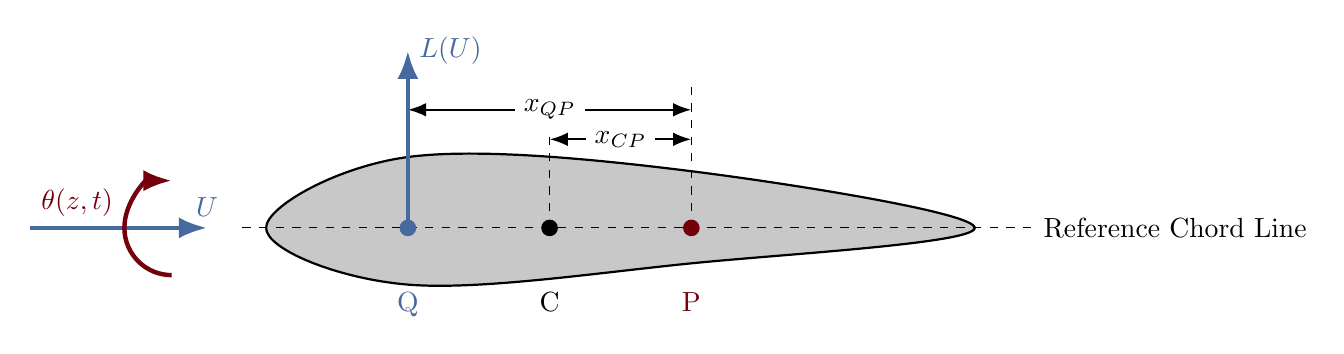
\begin{tikzpicture}[scale=1.5, >=Latex]
        % Airfoil shape (Consistent with 3D view roughly)
        % Normalized length 6 in drawing units
        \draw[thick, fill=UofSCLightGray] plot [smooth cycle, tension=0.6] coordinates {
            (0,0)           % LE
            (1.2, 0.6)      % Upper 1
            (3.6, 0.48)     % Upper 2
            (6,0)           % TE
            (3.6, -0.3)     % Lower 2
            (1.2, -0.48)    % Lower 1
        };
        
        \draw[dashed, UofSCBlack] (-0.2,0) -- (6.5,0) node[right] {Reference Chord Line};
        % Points Definitions scaled to fit this 0-6 chord
        % P at 2.4 (40%)
        % Q at 1.2 (20%)
        % C at 3.6 (60%)
        
        \coordinate (Q) at (1.2,0);
        \coordinate (C) at (2.4,0);
        \coordinate (P) at (3.6,0);
        % Distances (Offsets)
        \draw[<->, thick] ($(Q)+(0,1)$) -- ($(P)+(0,1)$) node[midway, fill=white] {$x_{QP}$};
        \draw[dashed] (P) -- ($(P)+(0,1.2)$);
        \draw[<->, thick] ($(P)+(0,0.75)$) -- ($(C)+(0,0.75)$) node[midway, fill=white] {$x_{CP}$};
        \draw[dashed] (C) -- ($(C)+(0,0.8)$);
        
        
        % Draw Points
        \fill[UofSCGarnet] (P) circle (2pt) node[below=7mm] {P};
        \fill[UofSCBlack] (C) circle (2pt) node[below=7mm] {C};
        \fill[UofSCAtlantic] (Q) circle (2pt) node[below=7mm] {Q};
        
        
        % Airspeed U
        \draw[->, ultra thick, UofSCAtlantic] (-2, 0) -- (-0.5, 0) node[above] {$U$};
        
        % Degrees of Freedom
        % Plunge w (at P, downward positive)
        \draw[->, ultra thick, UofSCAtlantic] (Q) -- ($(Q)+(0,1.5)$) node[right] {$L(U)$};
        
        % Pitch theta - smaller radius, more arc
        \draw[->, ultra thick, UofSCGarnet] ($(Q)+(-2,-0.4)$) arc (270:90:0.4) node[midway, above left] {$\theta(z,t)$};
        
% index (starting point f arc in x,y) arc (starting anlge:ending angle:radius) 
        
    \end{tikzpicture}
\end{figure}
\end{document}